\documentclass{beamer}

\usepackage[theme=dark,color=sysugreen,tpage=2]{sysubeamer}

\usepackage[scale=1.2]{ccicons}
\usepackage{CJKutf8}
\usepackage{hologo}
\usepackage{fontawesome}

% % 中文模式使用 XeLaTeX 编译器,并且使用 ctex 宏包,如:
% \usepackage[UTF8]{ctex}

\title[This is a Short Title]{This is a Long Sample Title and This is Not the Short Sample Title}
\subtitle{This is a sample subtitle}
\author{Your Name}
\school{School of Physics and Astronomy}
\date{\today}

\begin{document}

\maketitle

\begin{frame}[noframenumbering]{Copyright Notice}
    \begin{CJK*}{UTF8}{gbsn}
    \begin{itemize}
    \item 本模版基于~\href{https://creativecommons.org/licenses/by/4.0/deed.en}{\ccby} 协议开发,您可以自由地在任何媒介以任何形式复制、使用和修改本模版,只需给出适当的署名,详情请见:
    
    \url{https://creativecommons.org/licenses/by/4.0/deed.zh}
    \item 本模版的~ logo 由《中山大学视觉形象识别系统手册》里的素材导出,见:

    \url{http://home3.sysu.edu.cn/sysuvi/index.html}
    \item 物理与天文学院的~logo 见:
    
    \url{https://spa.sysu.edu.cn/zh-hans/article/290}
    \end{itemize}
    \end{CJK*}
\end{frame}

\setcounter{framenumber}{0}

\section{How to Use and Custom \texttt{sysubeamer}}

\begin{frame}[fragile]{How to Use}
\begin{columns}
    \column{0.5\textwidth}
     3 package options, the first one is set to default
    \begin{itemize}
        \item \texttt{theme}: theme mode, \texttt{light} or \texttt{dark}.
        \item \texttt{color}: the main color of theme, \texttt{sysugreen}, \texttt{sysured},\texttt{sysublack} or \texttt{spablue}.\par
        \textit{Notice: this option will affect the logo picture}.
        \item \texttt{tpage}: title page style, \texttt{1}, \texttt{2} or \texttt{3}, the results can be found at frame page \ref{tpage}.
    \end{itemize}
    \column{0.5\textwidth}
    \begin{block}{how to use \texttt{sysubeamer}}
\begin{lstlisting}[language=TeX]
\documentclass{beamer}
\usepackage[theme=dark,color=sysugreen,tpage=2]{sysubeamer}
\title[Short Title]{Normal Title}
\subtitle{Subtitle}     % optional
\author{Your Name}
\school{Your School}    % optional
\date{\today}
\begin{document}
\maketitle
\setcounter{framenumber}{0}
\section{Introduction}
\begin{frame}
    Your frame contents.
\end\{frame\}
\end{document}
\end{lstlisting}
    \end{block}
\end{columns}
\end{frame}

\begin{frame}[fragile]{How to Custom}
\begin{columns}
    \column{0.5\textwidth}
    \begin{itemize}
        \item the command \texttt{\textbackslash secsym} can custom your section symbol at table of contents;
        \item you can redefine the theme color by the command \texttt{\textbackslash themecolor} to your favorite color;
        \item if you want to use other logos, please redefine the commands as the right side codes, the meaning of these commands can be seen at frame page \ref{logo}.
    \end{itemize}
    \column{0.5\textwidth}
    \begin{block}{how to custom \texttt{sysubeamer}}
\begin{lstlisting}[language=TeX]
% wirte it at document preamble
\def\secsym{<symbol>}

\def\themecolor{<color>}

\def\logo{<path to logo.png>}
\def\motto{<path to motto.png>}
\def\horizontal{<path to horizontal.png>}
\def\vertical{<path to vertical.png>}
\def\updown{<path to updown.png>}
\end{lstlisting}
    \end{block}
\end{columns}
\end{frame}

\section{Basic Beamer Tricks}

\begin{frame}[allowframebreaks]{Basic Beamer Tricks}
    \begin{itemize}
        \item recommend that use the \texttt{align} environment for equations as shown below:
        \begin{align}
            v(t) = \kappa\left[\cos(f+\omega)+e\cos\omega\right] + v_0, \quad \text{with} \quad \kappa=\frac{(2\pi G)^{1/3}m\sin I}{T^{1/3}(M+m)^{2/3}\sqrt{1-e^2}}, \nonumber \\
            \text{where} \quad \tan(f/2)=\sqrt{\frac{1+e}{1-e}}\tan(u/2), \quad u-e\sin u = \frac{2\pi}{T}(t-\tau) \nonumber
        \end{align}
         \item recommend that use the \texttt{figure} environment to show your figures, seen at frame page \ref{table}. If you want to show multiple figure, please use the \texttt{subfigure} environment in \texttt{figure}.
        \item recommend that use the \texttt{booktab} package to show your tables, seen at frame page \ref{table}.
        \item recommend that use the \texttt{lstlisting} environment to show your codes, and don't forget to use the \texttt{[fragil]} option in \texttt{frame} environment, as shown at frame page \ref{listing}.
        \item if you want to split page, then recommend that use the \texttt{columns} environment to do it, seen at frame page \ref{splitandchinese}.
        \item if you want to Chinese language support in your slide, there are two ways to do it, seen at frame page \ref{splitandchinese}.
        
        \textit{Notice: if you use the} \texttt{ctex} \textit{package, don't forget to change your compiler to} \Hologo{XeLaTeX}.

        \item please try to use commands and frame options such as \texttt{\textbackslash pause}, \texttt{\textbackslash pause}, \texttt{allowframebreaks}, etc. as much as possible, in order to make your slide more smooth.
    \end{itemize}
\end{frame}

\section{Results of \texttt{sysubeamer}}

\begin{frame}[label=tpage]{Title page style}
    \centering
    \begin{figure}
        \centering
        \begin{subfigure}[b]{0.32\textwidth}
            
\includegraphics[width=\textwidth]{figure/tpage1.pdf}
            \caption{\texttt{tpage=1}}
        \end{subfigure}
        \begin{subfigure}[b]{0.32\textwidth}
            
\includegraphics[width=\textwidth]{figure/tpage2.pdf}
            \caption{\texttt{tpage=2}}
        \end{subfigure}
        \begin{subfigure}[b]{0.32\textwidth}
            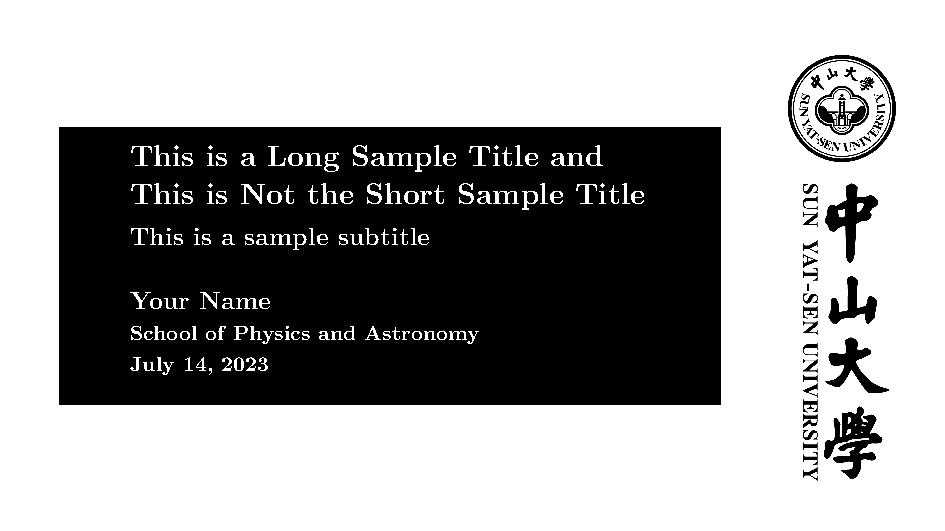
\includegraphics[width=\textwidth]{figure/tpage3.pdf}
            \caption{\texttt{tpage=3}}
        \end{subfigure}
        \caption{Title pages style based on the light and black theme.}
    \end{figure}
\end{frame}

\begin{frame}[label=logo]{Figure}{Logo picture}
    \centering
    \begin{figure}
        \begin{subfigure}[b]{0.72\textwidth}
            \centering
            \begin{subfigure}[b]{0.3\textwidth}
                \centering
                \includegraphics[width=\textwidth]{\logo}
                \caption{\texttt{\textbackslash logo}}
            \end{subfigure}
            \hspace{0.1\textwidth}
            \begin{subfigure}[b]{0.3\textwidth}
                \centering
                \includegraphics[width=\textwidth]{\updown}
                \caption{\texttt{\textbackslash updown}}
            \end{subfigure}
            \\
            \begin{subfigure}[b]{0.3\textwidth}
                \centering
                \includegraphics[width=\textwidth]{\horizontal}
                \caption{\texttt{\textbackslash horizontal}}
            \end{subfigure}
            \hspace{0.1\textwidth}
            \begin{subfigure}[b]{0.3\textwidth}
                \centering
                
\includegraphics[width=\textwidth]{\motto}
                \caption{\texttt{\textbackslash motto}}
            \end{subfigure}
        \end{subfigure}
        \hspace{0.08\textwidth}
        \begin{subfigure}[b]{0.18\textwidth}
            \centering
            \includegraphics[height=0.72\textheight]{\vertical}
            \caption{\texttt{\textbackslash vertical}}
        \end{subfigure}
    \end{figure}
\end{frame}

\begin{frame}[fragile,label=figure]{Figure}
    \begin{columns}
        \column{0.5\textwidth}
\begin{lstlisting}[language=TeX]
\begin{figure}
    \centering
    
\includegraphics[width=\textwidth]{logo/motto.png}
    \caption{The motto written by Mr. Sun Yat-sen: "Seeking truth, questioning, critical thinking, distinguishing, practicing."}
\end{figure}
\end{lstlisting}
        \column{0.5\textwidth}
        \begin{figure}
            \centering
            
\includegraphics[width=\textwidth]{logo/motto.png}
            \caption{The motto written by Mr. Sun Yat-sen: “Seeking truth, questioning, critical thinking, distinguishing, practicing.”}
        \end{figure}
    \end{columns}
\end{frame}

\begin{frame}[fragile,label=table]{Table}
    \begin{columns}
        \column{0.4\textwidth}
\begin{lstlisting}[language=TeX]
\begin{table}[htbp]
    \footnotesize
    \caption{2022 Winter Olympics medal table}
    \centering
    \begin{tabular}{ccrrrr}
        \toprule
        Rank & NOC & Gold & Silver & Bronze & Total\\ 
        \midrule
        1 & Norway & 16 & 8 & 13 & 37 \\
        2 & Germany & 12 & 10 & 5 & 27 \\
        3 & China & 9 & 4 & 2 & 15 \\
        \bottomrule
    \end{tabular}
\end{table}
\end{lstlisting}
        \column{0.6\textwidth}
        \begin{table}[htbp]
            \footnotesize
            \caption{2022 Winter Olympics medal table}
            \centering
            \begin{tabular}{ccrrrr}
                \toprule
                Rank & NOC & Gold & Silver & Bronze & Total \\ 
                \midrule
                1 & Norway & 16 & 8 & 13 & 37 \\
                2 & Germany & 12 & 10 & 5 & 27 \\
                3 & China & 9 & 4 & 2 & 15 \\
                \bottomrule
            \end{tabular}
        \end{table}
    \end{columns}
\end{frame}

\begin{frame}[fragile,t,label=listing]{Code: \texttt{corner} Plotting}
    \begin{columns}[t]
        \column{0.5\textwidth}
\begin{lstlisting}[language=TeX]
% \begin{frame}[fragile]
\begin{block}{\texttt{corner} plotting}
\begin{lstlisting}[language=Python]
# import corner
flat_samples = sampler.get_chain(discard=100, thin=15, flat=True)
fig = corner.corner(
    flat_samples,
    bins = 25,
    show_titles = True,
    labels = labels,
    plot_contours = True,
    quantiles = [0.16, 0.5, 0.84]
)
\end{block}
\|end\{lstlisting\}
\end{lstlisting}
        \column{0.5\textwidth}
        \begin{block}{\texttt{corner} plotting}
\begin{lstlisting}[language=Python]
# import corner
flat_samples = sampler.get_chain(discard=100, thin=15, flat=True)
fig = corner.corner(
    flat_samples,
    bins = 25,
    show_titles = True,
    labels = labels,
    plot_contours = True,
    quantiles = [0.16, 0.5, 0.84]
)
fig.savefig('corner.pdf')
\end{lstlisting}
        \end{block}
    \end{columns}
\end{frame}

\begin{frame}[fragile,label=splitandchinese]{Split Frame and Chinese Language Support}
    \begin{columns}
        \column{0.5\textwidth}
\begin{lstlisting}[language=TeX,caption=split the frame]
\begin{columns}
    \column{0.5\textwidth}
    contents 1
    \column{0.5\textwidth}
    contents 2
\|end\{columns\}
\end{lstlisting}
        \column{0.5\textwidth}
\begin{lstlisting}[language=TeX,caption=Chinese language support 1]
% \usepackage{CJKutf8}
\begin{CJK*}{UTF8}{gbsn}
    Chinese language support
\|end\{CJK*\}
\end{lstlisting}
\begin{lstlisting}[language=TeX,caption=Chinese language support 2]
% wirte it at document preamble
% use the XeLaTeX Compiler
\usepackage[UTF8]{ctex}
\end{lstlisting}
    \end{columns}
\end{frame}

\section{Summary}

\begin{frame}{Summary}
    \begin{itemize}
    \item any question about this template, please do not hesitate to contact me by below:
        \begin{itemize}
            \item \faEnvelope~~\href{mailto:yanghw8@mail2.sysu.edu.cn}{yanghw8@mail2.sysu.edu.cn}\
            \item \faQq~~929324613 (Group ID)
            \item \faGithub~~\url{https://github.com/yanghw8}
        \end{itemize}
    \item Best regards!
    \end{itemize}
\end{frame}

\backmatter

\end{document}
